\chapter{Mathématiques financières}

\section{Intérêts composés}

Un capital $c$ est placé sur un compte en banque à un taux $i$. Chaque année, le capital présent sur le compte augmente en fonction du taux d'intérêt. On obtient donc une suite que l'on peut définir ainsi (ou $c_n$ représente le capital à l'année $n$) :
$$
c_{n+1} = c_n + c_n \cdot i = c_n \cdot (1+i)
$$
Cette formule, selon le chapitre consacré aux suites, décrit une suite géométrique~\index{suite!géométrique} de raison $q = 1+i$. Ainsi la forme générale est donnée par la formule : $c_n = c_1 \cdot (1+i)^{n-1}$. Cependant, dans les exercices et dans la vie courante, il est plus intéressant de regarder le nombre d'années qui écoulées entre le dépôt du capital $c$ sur le compte et la valeur actuelle de ce dernier. Or si $c_1$ est le capital initial et que l'on laisse passer $n$ années, on doit chercher avec la formule non plus $c_n$, mais $c_{n+1}$. On obtient donc la formule


\begin{equation*}
\shadowbox{$
C = c \cdot (1+i)^n $}
\end{equation*}

\begin{equation*}
\mbox{ où } 
\begin{array}{lll}
C&=&\mbox{ capital d'arrivée}\\
c&=&\mbox{ capital de départ}\\
n&=&\mbox{ nombre d'années écoulées}\\
i&=&\mbox{ taux d'intérêt}\\
\end{array}
\end{equation*}

\section{Annuités}

On cherche à créer un patrimoine en déposant \textit{régulièrement} le même capital sur un compte. Si l'on dépose chaque année un montant $a$, on a 
$$
a \rightarrow a + a (1+i) \rightarrow a + a (1+i) + a(1+i)^2 \rightarrow \dots
$$
Il s'agit d'une série géométrique de raison $(1+i)$ et de terme initial $a$. Contrairement aux intérêts composés, il est plus adéquat de compter le nombre de versements pour retrouver la formule de la suite géométrique, d'où la formule :

\begin{equation*}
\shadowbox{$
A = a \cdot \frac{(1+i)^n-1}{i} $}
\end{equation*}

\begin{equation*}
\mbox{ où } 
\begin{array}{lll}
A&=&\mbox{ capital d'arrivée}\\
a&=&\mbox{ capital versé annuellment}\\
n&=&\mbox{ nombre de versements}\\
i&=&\mbox{ taux d'intérêt}\\
\end{array}
\end{equation*}

\textcolor{red}{Attention : le nombre de versements $=$ le nombre d'années $+1$}

\subsection{Mensualités}

Dans la vie courante, on trouve plus souvent des payements par mensualité. La formule est identique, mais les paramètres sont un peu modifiés :

\begin{equation*}
\shadowbox{$
M = m \cdot \frac{(1+i)^n-1}{i} $}
\end{equation*}

\begin{equation*}
\mbox{ où } 
\begin{array}{lll}
M&=&\mbox{ capital d'arrivée}\\
m&=&\mbox{ capital versé mensuellement}\\
n&=&\mbox{ nombre de versements}\\
i&=&\frac{\mbox{ taux d'intérêt}}{12}\\
\end{array}
\end{equation*}

\section{Remboursement d'une dette}

Toutes les formules données ci-après ne sont qu'une déduction des deux formules de base. Cependant, elles peuvent se montrer utiles pour éviter certains calculs.

On emprunte un certain montant $V$ auprès d'un établissement que l'on rembourses en $n$ versements annuels. \textcolor{red}{Le premiers remboursement commence une année après l'emprunt.}

On peut représenter la situation comme une balance entre deux comptes : l'un négatif et l'autre positif. On cherche donc après combien de versements les deux comptes sont à l'équilibre. Puisque le premier versement commence une année après l'emprunt, le nombre d'années d'intérêts composés pour la dette correspond au nombre de versements :

$$
V \cdot (1+i)^n = a \cdot \frac{(1+i)^n-1}{i}
$$

On divise par $(1+i)^n$ de chaque côté :

$$
V = a \cdot \frac{1-\frac{1}{(1+i)^n}}{i} 
$$

Grâce aux règles d'exposants on peut écrire $\frac{1}{(1+i)^n} = (1+i)^{-n}$ et on a donc la formule :

\begin{equation*}
\shadowbox{$
V = a \cdot \frac{1-(1+i)^{-n}}{i} $}
\end{equation*}

\begin{equation*}
\mbox{ où } 
\begin{array}{lll}
V&=&\mbox{ montant emprunté}\\
a&=&\mbox{ capital remboursé annuellment}\\
n&=&\mbox{ nombre de versements} = \mbox{ nombre d'années}\\
i&=&\mbox{ taux d'intérêt}\\
\end{array}
\end{equation*}

De manière identique, on peut calculer un remboursement mensuel en remplaçant 

\begin{equation*}
\mbox{ où } 
\begin{array}{lll}
V&=&\mbox{ montant emprunté}\\
a&=&\mbox{ capital remboursé mensuellement}\\
n&=&\mbox{ nombre de versements} = \mbox{ nombre d'années}\\
i&=& \frac{\mbox{ taux d'intérêt}}{12}\\
\end{array}
\end{equation*}

\section{Retraits réguliers}

On dispose d'un capital $X$ sur un compte en banque. Une année après, puis chaque année, on retire le même montant $a$. On cherche à connaître la valeur du compte après $n$ retraits.

Dans ce cas de figure, le nombre d'années et le nombre de retraits sont les mêmes. Il suffit de prendre la formules des intérêts composés et d'y soustraire celle des annuités. C'est comme si l'on avait deux comptes, l'un positif (capital) et l'autre négatif (retrait). Notre fortune se monte donc à la soustraction des deux montants :

\begin{equation*}
\shadowbox{$
Y = X(1+i)^n - a \cdot \frac{(1+i)^{n}-1}{i} $}
\end{equation*}

\begin{equation*}
\mbox{ où } 
\begin{array}{lll}
Y&=&\mbox{ capital restant}\\
X&=&\mbox{ capital de départ}\\
a&=&\mbox{ montant retiré annuellement}\\
n&=&\mbox{ nombre de versements} = \mbox{ nombre d'années}\\
i&=&\mbox{ taux d'intérêt}\\
\end{array}
\end{equation*}

\section{Exemple}

Parfois il est intéressant de représenter la situation graphiquement pour mieux savoir quelle(s) formule(s) utiliser. Une représentation standard (mais il en existe d'autres) consiste à utiliser un trait horizontal par année, une barre verticale s'il ne se passe rien, une croix pour un versement et un rond pour un retrait.

\begin{exemple}
Le premier janvier $2000$, puis chaque premier janvier, je dépose sur un compte à $2\%$ d'intérêt la somme de $1'500$chf, pour un total de cinq versements. Le premier janvier $2010$, puis chaque premier janvier jusqu'au premier janvier $2020$, je retire $500$chf de ce compte. Le premier janvier $2024$, j'achète une voiture à $7'000$chf. J'utilise le capital restant sur mon compte et j'emprunte le reste à un institut de prêt à rembourser en $24$ mensualités au taux de $7\%$. Quel sera le montant à payer chaque mois (versement le dernier jour du mois, premier versement le $31$ janvier) ?
\end{exemple}

On commence par faire une ligne qui représentera tout ce qui se passe sur le compte entre $2000$ et $2024$ :

\begin{center}
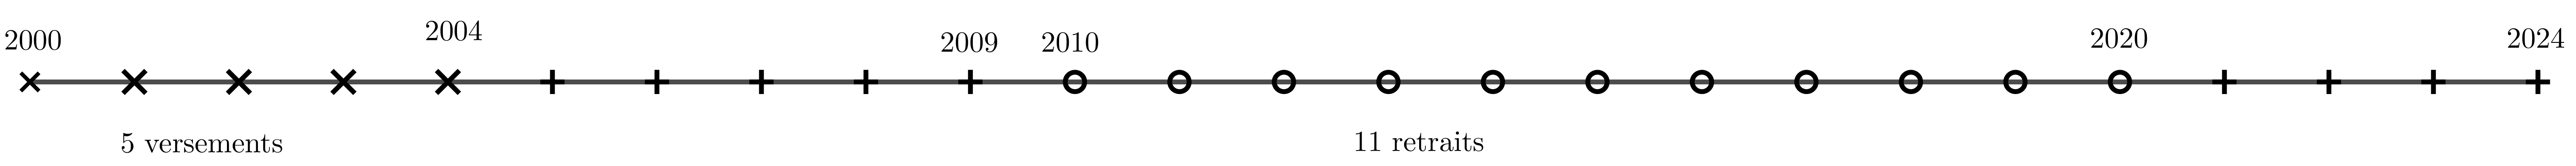
\includegraphics[width = \textwidth]{mathfin/ligneexemple.png}
\end{center}

On se sert de la ligne pour compter les informations manquantes (années, nombre de retraits). Puis on calcule la valeur du compte pour des années bien choisies :
\begin{enumerate}
\item[$2004$] Il s'agit d'une annuité :
$$
A = 1'500 \cdot \frac{1.02^5-1}{0.02} \simeq 7'806.05
$$
\item[$2009$] Si l'on veut utiliser ensuite la formule des retraits, il faut connaître la valeur du compte une année avant le premier retrait. Il s'agit d'un intérêt composé de $5$ ans :
$$
C = 7'806.05 \cdot 1.02^5 \simeq 8'618.50
$$
\item[$2020$] On utilise la formule des retraits pour $11$ retraits :
$$
Y = 8'618.50 \cdot 1.02^{11} - 250 \cdot \frac{1.02^11 - 1}{0.02} \simeq 4'631.70
$$
\item[$2024$] Il nous reste donc $4$ ans d'intérêts composés :
$$
4'631.70 \cdot 1.02^4 \simeq 5'013.50
$$
\end{enumerate}
À noter que pour chaque étape il convient de stocker la valeur dans la mémoire de la calculatrice et de n'arrondir que la réponse finale si l'on veut éviter des erreurs de centimes.

Dans la seconde partie du problème, un dessin semble superflu car il s'agit d'appliquer une formule de remboursement mensuel sans particularité. 

\begin{equation*}
\mbox{ Ainsi } 
\begin{array}{lll}
V&=&7'000-5'013.50 = 1'986.50\\
a&=&\mbox{ capital remboursé mensuellement} = \mbox{ inconnue}\\
n&=&24 \mbox{ mois}\\
i&=& \frac{0.07}{12}\\
\end{array}
\end{equation*}

On a donc :

$$
1'986.50 = a \cdot \frac{1-1.0058\overline{3}^{-24}}{0.0058\overline{3}} \Longrightarrow a \simeq 186.95\mbox{chf}
$$

En bref, ce genre de donnée peut paraître inabordable, mais si l'on découpe correctement le problème, chacune des étapes suit une formule.
\section{Exercice}

\begin{exercice}
Quel est le capital qui, placé à intérêts composés et à $5 \%$ pendant 10 ans, est devenu Fr. 12'640.— ?
\end{exercice}

\begin{exercice}
Une somme de Fr. 10'000.— placée à intérêts composés est devenue Fr. 20'360.— après 15 ans. Calculer le taux des intérêts composés.
\end{exercice}

\begin{exercice}
Une somme de Fr. 40'000.— placée à intérêts composés à $4.5 \%$ est devenue Fr. 67'835.70, pendant combien d’années a-t-elle été placée ?		
\end{exercice}

\begin{exercice}
A quel taux faudrait-il placer une somme de Fr. 10'000.—, à intérêts simples, pour qu’après 6 ans elle eût rapporté autant que cette même somme placée à intérêts composés à $4 \%$ pendant le même temps ?	
\end{exercice}

\begin{exercice}
Pendant combien d’années faudrait-il placer un capital à intérêts composés à $4.5 \%$ pour tripler ce capital ?
\end{exercice}

\begin{exercice}
En payant une dette douze ans avant son échéance, on a obtenu une réduction de Fr. 2'570.62. Calculer la valeur nominale de la dette et la somme payée pour l’acquitter. Le taux des intérêts composés est de 5 %.
\end{exercice}

\begin{exercice}
Un capital de Fr. 1'025'000.— a été placé à $4 \%$ pendant 5 ans. A ce moment-là, son propriétaire retire pour ses besoins personnels Fr. 222'069.20. Le montant restant est replacé au taux de $6 \%$ pendant 10 ans. 
Quel est le capital après ce temps de placement ?
\end{exercice}

\begin{exercice}
Un de mes ancêtres a placé Fr. 100.—. Ce montant est devenu Fr. 49'410'548.—. Combien de temps l’ai-je placé, si le taux de capitalisation a été de $6 \%$ ?
\end{exercice}

\begin{exercice}
Mon père a remis une certaine somme dont il disposait le jour de ma naissance à sa banque. Le 01.01.2003 je me retrouve avec un capital de Fr. 30'000.— et j’ai 30 ans. Le taux moyen du placement a été de $5,5 \%$.
Quel montant mon père a-t-il placé ?
\end{exercice}

\begin{exercice}
Le taux moyen de renchérissement du coût de la vie a été dans un certain pays au cours des dix dernières années de $5.8 \%$ annuellement. Un ouvrier gagnait Fr. 4'267.80 au 1er janvier 1993 dans une entreprise qui a toujours indexé intégralement ses salaires. Quel est son salaire au 1er janvier 2003 ?
\end{exercice}

\begin{exercice}
Tu disposes de deux capitaux. Le premier atteint un montant de Fr. 2'198'852.— et le second se monte à Fr. 2’000'000.—. Tu places le premier à $5 \%$ et le second à $6 \%$. Après combien de temps le deuxième capital sera-t-il d’un montant égal au premier ?
\end{exercice}

\begin{exercice}
Un capital de Fr. 80'000.— a été placé comme suit :
\begin{itemize}
\item pendant  5 ans,  à $7 \%$
\item puis, pendant 6 ans, à $7.5 \%$
\item puis, pendant 11 ans, à $8 \%$
\item puis enfin, pendant 3 ans, à $4 \%$
\end{itemize}
Combien retirera-t-on après ces 25 ans ? Si pendant tout le placement, on avait voulu avoir un taux unique de rendement et toucher en finale le même montant, quel aurait dû être ce taux ?
\end{exercice}

\begin{exercice}
Un capital de Fr. 1'000'000.— est devenu Fr. 2'000'000.— après 10 ans. Quel a été le taux de placement ?
\end{exercice}

\begin{exercice}
On place à intérêts composés une somme de Fr. 250'000.— à $8 \%$ pendant 5 ans; puis, on déplace le montant obtenu auprès d’une autre banque qui a trouvé un placement rétribué à $10 \%$. Après 6 nouvelles années, nous retirons Fr. 250'751.—. Que reste-t-il sur notre compte après ce retrait ?
\end{exercice}

\begin{exercice}
Si, le 1er janvier de l'an 1, un Romain avait placé pour toi à $0.5 \%$ l’équivalent de Fr. 100.—, de quelle somme disposerais-tu le 1er janvier 2001 ?
\end{exercice}

\begin{exercice}
En remboursant une dette de Fr. 25'000.— trois ans avant son échéance on a obtenu un escompte de Fr. 4'303.75. Calculer le taux des intérêts composés.
\end{exercice}

\begin{exercice}
On dispose de Fr. 500'000.— à placer. Deux banquiers contactés te proposent ceci :
\begin{itemize}
\item 1e banquier : Placement de  Fr. 500'000.–– pendant 10 ans à $5 \%$, puis pendant 5 ans à $7 \%$
\item 2e banquier :  1e  tranche de 200'000.–– pendant 15 ans à $5 \%$
2e  tranche de 300'000.–– pendant 10 ans à $6 \%$, puis pendant 5 ans à $5 \%$
\end{itemize}
Quelle proposition choisirais-tu si tu veux que ton capital te rapporte le maximum ? Quel sera ton gain si tu choisis la meilleure solution ?
\end{exercice}

\begin{exercice}
Une somme de Fr. 100'000.— est payable dans 10 ans. Déterminer sa valeur :
\begin{itemize}
\item aujourd’hui
\item dans 3 ans
\item dans 15 ans
\item dans 12 ans et 7 mois
\end{itemize}
Taux annuel de $3.5 \%$.
\end{exercice}

\begin{exercice}
Le 1er janvier 1990 une personne a placé la somme de Fr. 10'000.— sur compte d'épargne. Le 1er janvier 1996 elle effectue un deuxième placement sur ce même compte. Calculer le montant de ce deuxième versement sachant qu'au 31 décembre 2002 le montant du compte est de Fr. 36'774.—.
\end{exercice}





\subsection{Placements}

\begin{exercice}
Quel est le montant de l’annuité que je dois verser pour obtenir un capital de Fr. 10'253'224.— au moment du vingtième versement, si le taux est de $6.28 \%$ ?
\end{exercice}

\begin{exercice}
Après avoir placé 20 annuités à intervalle d’une année, on veut obtenir un capital de Fr. 160'000.—. Le taux des intérêts composés étant de $6 \%$, quelle doit être la valeur de l’annuité versée chaque année si le capital doit être constitué un an après le dernier versement ?
\end{exercice}

\begin{exercice}
Au 01.01.1993, j’ai décidé de verser le 1er mars de chaque année un montant de Fr. 12'000.— sur un compte qui rapporte du $5.05 \%$.
	Le 1er mars 1993, j’ai 21 ans. Quel montant sera-t-il à ma disposition le jour de mes 60 ans ?


Combien devrais-je placer chaque année à $4\frac{1}{4} \%$ pour toucher au moment du vingt-quatrième versement Fr. 101'911.85  ?
\end{exercice}

\begin{exercice}
Combien ai-je effectué de versements si j’ai versé chaque année Fr. 5'531.10 et que j’ai retiré après un certain temps Fr. 120'000.— ? (taux $5 \%$)
\end{exercice}

\begin{exercice}
Le 15 mars 1988 Monsieur Vittorio Rossi  a gagné à la loterie la somme de Fr. 1'455'800.—. Le fisc a retenu à la source Fr. 509'000.—.
Monsieur Rossi a placé le reste de son gain sur un compte bancaire au taux de $5 \%$.

Le 15 mars 1990, il a retiré Fr. 65'000.— pour l’achat d’une voiture.
Le 15 mars 1993, il a retiré Fr. 25'000.— pour un grand voyage à l’occasion de ses 60 ans.

Monsieur Rossi étant indépendant, il n’a pas cotisé à une de caisse de retraite. Il souhaite conserver le solde du compte comme source de revenu pour ses vieux jours.
Sachant qu’il aura 65 ans le 15 mars 98, combien aura-t-il mis de côté pour ses vieux jours à ce moment-là ?
\end{exercice}

\begin{exercice}
Un indépendant a prévu de créer sa propre caisse de retraite. Pour se faire, il a placé chaque année Fr. 3'600.— et ceci à 20 reprises, puis Fr. 4'800.— à 10 reprises et enfin 5 versements de Fr. 6'000.—.
De quelle somme dispose-t-il au moment du dernier versement, si le taux a été constant à $4.05 \%$ ?

Du 1er janvier 1960 au 1er janvier 1996, un individu a versé des annuités constantes pour avoir Fr. 3'259'702.80 au 1er juillet 2005. Si le taux a été constant $4.25 \%$, calculer le montant de l’annuité versée par cette personne.
\end{exercice}

\begin{exercice}
En examinant un placement en francs suisses à l’étranger, on constate les mouvements de capitaux suivants :

1er janvier 1970 : ouverture du compte : versement de Fr. 240'000.—	
1er janvier 1975 : retrait du compte Fr. 20'000.—	
1er janvier 1983 : versement sur le compte Fr. 360'000.—	
1er janvier 1985 : versement sur le compte Fr. 240'000.—	
1er janvier 1992 : retrait du compte Fr. 50'000.—

Si les taux d’intérêts appliqués ont été de :
$8 \%$ du 1er janvier 1970 au 31 décembre 1977 
$9 \%$ du 1er janvier 1978 au 31 décembre 1982
$10 \%$ du 1er janvier 1983 à ce jour.

Calculer la somme indiquée par ce compte au 1er janvier 1993. 
\end{exercice}

\begin{exercice}
Du 1er janvier 1950 au 1er janvier 1963 : 	versements de Fr. 10'500.— chaque 1er janvier
A partir du 31 mars 1967 : 		12 versements de Fr. 12'000.— chaque 31 mars
Le 1er juillet 1971 : 		retrait de Fr. 25'000.—
Du 1er juillet 1970 au 1er juillet 1981 : 	versements de Fr. 7'000.— chaque 1er juillet
Le 1er octobre 1985 : 		retrait de Fr. 12'500.—

Combien y a-t-il sur le compte le 31 décembre 1990 ? (taux $3 \%$)
\end{exercice}

\begin{exercice}
Un financier a versé à sa caisse de retraite :
le 1er janvier 1997 un montant global de Fr. 100’000.—,
versements du 1er juillet 1998 au 1er juillet 2010 chaque 1er juillet de Fr. 10’000.—,
le 31 décembre 2012, il retire Fr. 331’000.—.

Combien lui reste-t-il à prélever au 1er janvier 2013, si le taux de rendement est de $3\frac{3}{4} \%$ ?
\end{exercice}

\subsection{Emprunts}

\begin{exercice}
Un emprunt de Fr. 250'000.— doit être remboursé en 18 annuités constantes, la première fois une année après l’emprunt. Si le taux est de $4.75 \%$, combien devra-t-on payer annuellement ?
\end{exercice}

\begin{exercice}
A combien se montait initialement un emprunt, si nous avons remboursé 26 montants de Fr. 22'000.— annuellement et si le taux était de $8\frac{1}{3} \%$ ?
\end{exercice}

\begin{exercice}
Combien de remboursements avons-nous effectué, si le capital emprunté se montait à Fr. 200'000.— et si nous avons versé chaque année Fr. 29'705.55 avec un taux de $4 \%$ ?
\end{exercice}

\begin{exercice}
Une personne place le même jour à intérêts composés deux capitaux s’élevant ensemble à Fr. 25'000.—, le premier à $4 \%$ et le deuxième à $5 \%$. Au bout de deux ans, elle en retire la valeur acquise qui se monte à Fr. 27'249.—. Quel était le montant de chaque capital ?
Après avoir retenu Fr. 2'249.— pour s’acquitter d’une dette, cette personne prête le restant à un ami qui s’engage à en faire le remboursement par 3 annuités dont la première est payable dans un an.
Déterminer le terme de l’annuité, le taux de l’intérêt composé étant de $5 \%$. 
\end{exercice}

\begin{exercice}
Un père de famille a 30 ans et décide d’investir Fr. 500'000.— dans l’achat d’un logement. Il dispose de Fr. 70'000.— de fonds propres et emprunte le solde. Pour ce solde, la banque contactée, lui a prêté contre une garantie hypothécaire les $\frac{3}{4}$ en premier rang au taux de $5.5 \%$ et le $\frac{1}{4}$ en deuxième rang au taux de $6 \%$.
Après avoir effectué différents calculs, ce citoyen opte pour les conditions de remboursement suivantes :
Remboursement prioritaire par 8 annuités constantes de la dette en deuxième rang, première annuité lorsque le père de famille a 31 ans.
Remboursement ensuite de la dette en premier rang par des annuités constantes (la première fois une année après la fin du paiement des 8 annuités; la dernière fois le jour de ses 65 ans).
Quel sera le montant de l’annuité pour le remboursement du prêt en deuxième rang ?
Quel sera le montant de l’annuité pour celui du prêt en premier rang ?
Quelle somme devra encore le père de famille le jour de ses 55 ans ?
\end{exercice}

\subsection{Retraits et divers}

\begin{exercice}
Le 1er mars 2011, j’atteindrai mes 60 ans et j’estime que mon capital rentier atteint Fr. 384'000.—. Quelle somme puis-je retirer annuellement de ce capital la première fois une année après mes 60 ans pour qu’après 26 retraits, il ne me reste rien ? (taux $10.15 \%$) 
\end{exercice}

\begin{exercice}
J’ai eu la chance de toucher Fr. 240'000.— d’un de mes oncles. Sur cet héritage, l’Etat du Valais a prélevé un impôt sur les successions et les donations de $10 \%$. J’ai placé le solde sur un compte à $8.1 \%$.
	Je prélève une année après mon héritage Fr. 20'000.—, puis Fr. 30'000.— 5 ans jour pour jour après le versement des Fr. 240'000.—. De quel montant disposerai-je 20 ans après l’héritage si le taux reste constant à $8.1 \%$ ?
\end{exercice}

\begin{exercice}
Un employé de banque a placé chaque année et 27 fois de suite Fr. 2'773.55. Il laisse s’écouler une année, puis retire chaque année 27 fois Fr. 7'000.—. Que lui reste-t-il après ces opérations, le taux étant de $4\frac{1}{4} \%$ ?
\end{exercice}

\begin{exercice}
Je dispose de Fr. 123'456.—. Que me reste-t-il sur ce capital placé à $7\%$, si je retire, une année après le versement à la banque des Fr. 123'456.—, seize montants annuels fixes de Fr. 12'000.— ?
\end{exercice}

\begin{exercice}
Un employé a placé chaque année et 25 fois de suite une somme de Fr. 12'000.— dans une banque. Il laisse ensuite s’écouler 10 ans, puis, dès l’année suivante, il retire chaque année, d’abord 10 fois Fr. 30'000.—, puis 5 fois Fr. 20'000.––. Que lui reste-t-il alors en banque ? (taux $5.25 \%$)
\end{exercice}

\begin{exercice}
Une forêt contient 80'000 m3 de bois et s’accroît chaque année de $3 \%$. Combien de m3 de bois seront-ils à disposition pour la coupe après 30 ans. Une année après ces 30 années, le forestier décide de couper chaque année 10'000 m3. Après combien de temps la forêt sera-t-elle entièrement rasée ?
\end{exercice}

\begin{exercice}
Un père de famille désire acheter un petit immeuble à rénover à Martigny. Le propriétaire de cette bâtisse est d’accord de la lui céder pour Fr. 150'000.—. Les frais de notaire et d’inscription au RF sont à la charge de l’acquéreur et représente le $2.5 \%$ du prix d’achat; en plus, à sa charge, des travaux urgents de transformations devront être effectués. Les devis estimatifs de ces travaux sont résumés dans le tableau suivant :


1	Recrépissage des façades	Fr.  25'000.––
2	Dépose et pose de tapisseries neuves	Fr.  10'000.––
3	Changement du bloc de cuisine	Fr.  20'000.––
4	Isolation thermique et phonique	Fr.  15'000.––
5	Aménagement des combles	Fr.  12'500.––
6	Pose d’un « vélux »	Fr.    1'250.––
7	Autorisation communale	Fr.       500.––


Ce citoyen prévoit en plus une somme de Fr. 12'000.— pour des imprévus. Il dispose en banque de fonds propres se montant à Fr. 75'500.—.

Combien devra-t-il emprunter à la banque pour financer cette acquisition ? 

Il désire, pour des raisons personnelles, amortir la dette contractée auprès de la banque en 11 annuités constantes. Combien paiera-t-il s’il commence à amortir la dette une année après l’achat et la fin des travaux si le taux du prêt est de $5\frac{3}{4} \%$ ?

Au moment du cinquième versement, il a la chance de toucher un héritage qui lui permet d’effectuer un versement complémentaire à l’annuité de Fr. 12'500.—.
Quel montant devra-t-il payer ensuite comme nouvelle annuité s’il désire finir de payer la dette comme prévue en 11 versements ?
\end{exercice}

\begin{exercice}
On veut amortir un emprunt de Fr. 320'000.— en 15 ans par des annuités constantes. Le remboursement commence une année après le prêt. Après 8 ans, on décide d’augmenter l’annuité calculée de Fr. 5'500.— par année. Combien d’annuités sont nécessaires pour finir de payer notre dette si le taux pratiqué est de $7 \%$ ? (Arrondir la dernière annuité)
\end{exercice}

\begin{exercice}
Une personne a emprunté Fr. 300'000.— à rembourser en 10 versements annuels. Après avoir effectué 5 versements, elle désire s’acquitter du reste par un versement unique. Quel est le montant de ce versement si le taux est de $4.5 \%$ ?
\end{exercice}

\begin{exercice}
Un particulier a emprunté auprès de sa banque, un montant de Fr. 150'000.— à $4\frac{3}{4} \%$ à rembourser en 20 ans par des annuités constantes. Le remboursement commence une année après le prêt. Après 9 versements le taux change et passe à $4 \%$. En supposant que cet individu continue à rembourser le même montant initialement prévu, combien d’annuités sont nécessaires pour finir de payer sa dette ? (Arrondir la dernière annuité)
\end{exercice}

\begin{exercice}
Monsieur Favre a versé, depuis le jour de ses quarante-deux ans, à chaque date d’anniversaire et jusqu’à l’âge de 64 ans compris, la somme de Fr. 5’000.— sur un compte d’épargne pour se constituer un capital pour sa retraite. 
Dès le jour de ses 68 ans, il retire chaque année à sa date d’anniversaire la somme de Fr. 30’000.—. (Taux des intérêts composés : $3.75 \%$)

Jusqu’à quel âge pourra-t-il retirer entièrement cette somme ?

Quelle somme pourra-t-il alors encore retirer une année après avoir effectué le dernier retrait entier de Fr. 30’000.— ?
\end{exercice}

\begin{exercice}
Monsieur et Madame Blanc ont versé chaque année de 1970 à 1990 une certaine somme sur un compte à $2.5 \%$. Au moment du dernier versement, ils obtiennent une somme de Fr. 67958,20

a.	Combien ont-ils versé chaque année ?

Ils laissent ensuite cet argent à la banque et font les retraits suivants :

En 1995 : Fr. 6'000.–– pour un voyage
En 1997 : Fr. 12'000.–– pour l'achat d'une voiture
A partir de 1998, ils retirent annuellement la somme de Fr. 5500.––

b.	En quelle année pourront-ils retirer le dernier retrait entier de Fr. 5'500.–– ?

c.	Quelle somme pourront-ils encore retirer une année après avoir effectué le dernier retrait entier de Fr. 5500.–– ?
\end{exercice}

\begin{exercice}
Jacques Fischer a versé du 1er janvier 1976 au 1er janvier 1986, chaque année une somme de Fr. 15'000.— sur un compte d’épargne au taux de $1.75 \%$.
Son ami André Bumann a également épargné du 1er janvier 1979 au 1er janvier 1990, chaque année une somme de Fr. 12'000.— sur un compte d’épargne au taux de $1.5 \%$.
Le 1er juillet 1992, Jacques et André décident de mettre en commun le $75 \%$ de leurs économies sur un compte à $2 \%$.

Combien ont-ils sur leur compte commun au 1er juillet 1992 ?

Le 1er janvier 1994, ils achètent une surface commerciale pour la somme de Fr. 900'000.—. Pour cela ils utilisent leur compte commun et empruntent le solde au taux de $5.5 \%$. 

Quel est le montant de l’emprunt ?

La banque leur propose de rembourser leur dette en 20 annuités constantes à partir du 1er janvier 1997.

Quel est le montant de l’annuité versée ?

Après avoir effectué 13 versements, les deux amis reçoivent un héritage qui leur permet de rembourser entièrement la dette. 

Quelle est la somme versée ?
\end{exercice}
